%-----------------------------------------------------------------------------
%
%               Template for sigplanconf LaTeX Class
%
% Name:         sigplanconf-template.tex
%
% Purpose:      A template for sigplanconf.cls, which is a LaTeX 2e class
%               file for SIGPLAN conference proceedings.
%
% Guide:        Refer to "Author's Guide to the ACM SIGPLAN Class,"
%               sigplanconf-guide.pdf
%
% Author:       Paul C. Anagnostopoulos
%               Windfall Software
%               978 371-2316
%               paul@windfall.com
%
% Created:      15 February 2005
%
%-----------------------------------------------------------------------------


\documentclass[preprint,nocopyrightspace]{sigplanconf}

% The following \documentclass options may be useful:

% preprint      Remove this option only once the paper is in final form.
% 10pt          To set in 10-point type instead of 9-point.
% 11pt          To set in 11-point type instead of 9-point.
% authoryear    To obtain author/year citation style instead of numeric.

\usepackage{graphicx}
\usepackage{amsmath}
\usepackage{listings}
\usepackage{caption}
\usepackage{algorithm}
%\usepackage{algorithmicx}
\usepackage{algpseudocode}

\begin{document}

\lstset{language=Haskell,basicstyle=\ttfamily,captionpos=b}

\special{papersize=8.5in,11in}
\setlength{\pdfpageheight}{\paperheight}
\setlength{\pdfpagewidth}{\paperwidth}

%\conferenceinfo{CONF 'yy}{Month d--d, 20yy, City, ST, Country} 
%\copyrightyear{20yy} 
%\copyrightdata{978-1-nnnn-nnnn-n/yy/mm} 
%\doi{nnnnnnn.nnnnnnn}

% Uncomment one of the following two, if you are not going for the 
% traditional copyright transfer agreement.

%\exclusivelicense                % ACM gets exclusive license to publish, 
                                  % you retain copyright

%\permissiontopublish             % ACM gets nonexclusive license to publish
                                  % (paid open-access papers, 
                                  % short abstracts)

%\titlebanner{banner above paper title}        % These are ignored unless
%\preprintfooter{short description of paper}   % 'preprint' option specified.
\toappear{Final paper for Comp150-05: Advanced Functional Programming}
\title{Random Strictness at Source Level}
%\subtitle{Subtitle Text, if any}

\authorinfo{Diogenes Nunez}
           {Tufts University}
           {dan@cs.tufts.edu}
%\authorinfo{Name2\and Name3}
%           {Affiliation2/3}
%           {Email2/3}

\maketitle
\thispagestyle{plain}
\pagestyle{plain}
%\cfoot{\thepage}
\begin{abstract}
Haskell is a lazy language which can cause slowdown due to the creation of thunks. Strictness can force evaluation of expressions and avoid the cost of thunks. However, programmers adding it into source code for performance may not know where to start. This case worsens if it is code they did not write. We introduce a genetic algorithm with the purpose of developing a faster program through adding strictness to the source code.
\end{abstract}

%\category{CR-number}{subcategory}{third-level}

% general terms are not compulsory anymore, 
% you may leave them out
%\terms
%term1, term2

%\keywords
%keyword1, keyword2

\section{Introduction}\label{sec:intro}

Haskell is lazy. Consider this function
\begin{lstlisting}[label={lst:repl}]
-- Create infinite list
repeat :: a -> [a]

replicate :: Int -> a -> [a]
replicate n x = take n xs
                where xs = repeat x
\end{lstlisting}
In an eager language, \lstinline!xs! would be evaluated immediately. This results in a nonterminating function. However, a lazy language would only evaulate \lstinline!xs! when required. Even then, the expression only gets what it needs. Therefore, only \lstinline!n! items are required and processed.

How does Haskell do this? To explain, consider this function
\begin{lstlisting}[label={lst:f}]
f :: Int -> [Int]
f n = replicate n n
\end{lstlisting}
Consider the application \lstinline!f (x+1)!. Haskell creates a closure on the heap that contains the unevaluated expression \lstinline!x+1!. This is a thunk. The function \lstinline!f! then gets a pointer to that. When the value within is needed, Haskell traverses to the thunk and evaluates it, potentially writing something back to the heap. Note that an eager language would not have written the thunk in the first place, avoiding both the additional write and the read.

How well does this scale? Suppose we had a large group of thunks. The larger the group, the more memory pressure applied to the application. This leads to more frequent garbage collections and overall slowdown. In some cases, we may have programs that crash due to a lack of memory. We might save some overall time and space by evaluating some of those thunks early. Haskell has notation to force eager evaluation, the bang.
\begin{lstlisting}[label={lst:fstrict}]
f :: Int -> [Int]
f !n = replicate n n
\end{lstlisting}

Now, we force Haskell to evaluate \lstinline!n! and pass that value on to \lstinline!f!. \lstinline{n} is evaluated eagerly. Here, no thunk is created and if \lstinline{n} is no longer used in the program, the garbage collector can throw it away. We have saved some time and space. We say that \lstinline!f! is now strict in \lstinline!n! and the process of forcing eager evaluation is adding strictness to the program.

Now consider a far more complicated program, spreading across multiple files. We must ask ourselves two questions. First, where do we start adding strictness? Here we only had one function, so the process was simple. With many functions, some recursive, adding strictness could cause problems, like nontermination. Second, when do we stop? Adding too much strictness can cause excess memory pressure. This would be no different, or worse, than the completely lazy version. We need to find a balance between lazy and eager in order to improve the program.

In this paper, we discuss a program that searches the space of strict programs using a genetic algorithm to find a faster version of a given program. Section~\ref{sec:back} covers the background of strictness analysis and related work. Section~\ref{sec:arch} covers the program. Section~\ref{sec:expr} discusses some experiments. Section~\ref{sec:conc} concludes the paper.

\section{Background}\label{sec:back}
Strictness analysis looks at a function with $n$ arguments and asks whether the $i^{\text{th}}$ argument can be made strict. Programmers and compilers use the results of such an analysis to make their programs strict. The problem itself is hard. Part of strictness analysis is asking whether the program will terminate, also known as the halting problem. Work in the field focuses on approximating the analysis.

Peyton Jones and Partain created a simple strictness analyzer that would run on GHC Core.\cite{pjones} The analysis was an approximation of finding fixpoints of functions. They used a ``widening'' operator on functions, removing some constraints and finding those fixpoints. As a static analysis, it will flag some functions as non-terminating when made strict on some arguments. Furthermore, they note their analyzer does not deal with non-flat structures and recursive functions. The work presented here does not ignore these two items. As long as the algorithm knows strictness can be annotated, it has a chance of doing so.

Schrijvers and Mycroft worked on a type inference algorithm that kept track of the effects of functions, both deterministic and non-deterministic \cite{mycroft, wadler}. They use this to bring data flow to strictness analysis. Just like Peyton Jones and Partain, they consider flat data. Again, we do not ignore data so long as the algorithm knows it can make the data strict.

Jensen et. al. moved to an analyzer on GHC Core that handled higher-order functions and polymorphism \cite{jensen}. They also approximate fixpoints. However, they make no note in their paper on using the results on functions. Their work incorporated the theoretic foundations from Wadler\cite{wadler} to do this. Our work differentiates itself from both Peyton Jones and Jensen by working closer to sugared source code than GHC Core. This allows us to output code for a Haskell user that they can learn from, rather than giving GHC Core back or just compiling straight to machine code.

\section{Architecture}\label{sec:arch}
\begin{figure}[t]
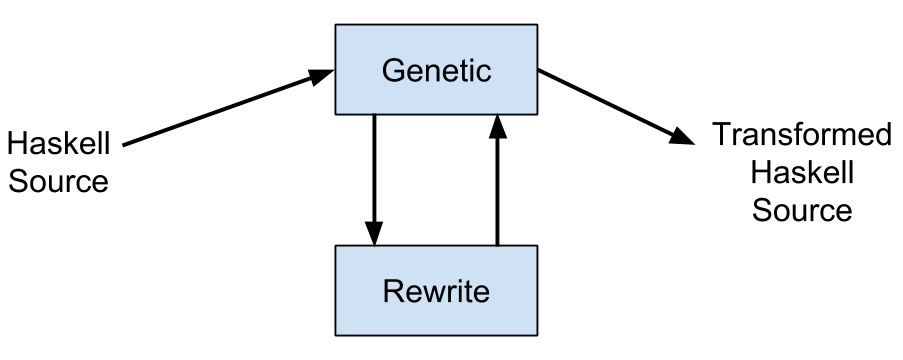
\includegraphics[width=\columnwidth]{modules.png}
\caption{General architecture}
\label{fig:arch}
\end{figure}
The program has three components, as shown in Figure~\ref{fig:arch}. The Rewrite module deals with adding strictness to the source code itself. The Genetic module is the core of the program, deciding when and where to add the strictness. It uses the Rewrite module to edit the source code. We give it the Haskell source code and we get back Haskell source code. The rest of this section discusses the modules in more detail.
\subsection{Rewrite}
This module takes in sugared Haskell source code, creates an abstract syntax tree, transforms it, and prints it back as sugared Haskell code without comments. We use the \lstinline!haskell-src-exts! package to get the abstract syntax tree and print it back to readable source~\cite{hsrcext}. It exposes three functions, \lstinline!flipBang!, \lstinline!flipRandomBang!, \lstinline!placesToStrict!.

\lstinline!flipBang! takes in a \lstinline!FilePath! to the file, a \lstinline!String! containing the whole program, and an \lstinline!Int! that denotes which declaration in the program to add or remove strictness. If the program was entered with strictness at that location, it will leave without it and vice-versa. \lstinline!flipRandomBang! does the same, but in at a random location in the program. Finally, \lstinline!placesToStrict! gets the file path and program as input and returns the number of places one can place strictness.

All three functions perform the same steps and traversal. To begin, they retrieve the module the program given describes. We use \lstinline!parseFileContentsWithMode! to extract the abstract syntax tree of the module while enabling the compiler flag \lstinline!-XBangPatterns! and the Haskell 2010 language. 

From there, we can get a list of declarations. This includes all functions declared in the file. The package labels them as \lstinline!FunBind!s. Each one contains a list of parameters, typed \lstinline!Match!. Each of those contains contains \lstinline!Pat!, or patterns. \lstinline!Pat! contains multiple datatypes, but two concern us in this implementation. One is \lstinline!PVar!, a parameter or variable declaration in a \lstinline!where! clause. The other is \lstinline!PBangPat!, something with strictness applied to it. \lstinline!flipBang! and \lstinline!flipRandomBang! will either replace a \lstinline!PVar! with a \lstinline!PBangPat! or vice-versa. \lstinline!placesToStrict! increments its counter.

\subsection{Genetic Algorithm}
This module is the driving force behind the program. Its purpose is to run the genetic algorithm, exploring the space of programs, choosing some, and running them to determine the best. The rest of this subsection describes the module.
\subsubsection{Datatypes and Operations}
\begin{lstlisting}[float,caption=Datatypes and operations in Genetic module,label={lst:genetic},frame=single]
data Strand = {  path    :: FilePath
               , program :: String
               , vec     :: Integer
               , size    :: Int
              }

data Genes = { getStrands :: [Strand] }

mutate :: Genes -> Genes
merge :: Genes -> Genes -> Genes
fitness :: Int -> Float -> Genes -> 
           IO Float
\end{lstlisting}
\begin{lstlisting}[float,caption=Example program,label={lst:example},frame=single]
replicate' :: Int -> a -> [a]
replicate' !n x = take n xs
                  where xs = repeat x
\end{lstlisting}

Listing~\ref{lst:genetic} lists the important datatypes and operations used in the module. \lstinline!Strand! is used to describe a single file. It contains the path to the file, the program in a \lstinline!String!, a bit vector represented by an \lstinline!Integer!, and an \lstinline!Int! recording the size of that bit vector. Each bit in the vector, starting from the least significant, corresponds to a location in the program where the Rewrite module can place strictness. $0$ means there is no strictness. $1$ means there is. This allows us to keep track of the status of the file without digging into the program itself. For example the vector for the program in Listing~\ref{lst:example} is $001$. We record the size of the vector since \lstinline!bitSize! of an \lstinline!Integer! is undefined in \lstinline!Data.Bits!.

\begin{figure}[t]
\begin{algorithmic}
\Function{mutateSet}{\lstinline!Strand! s, \lstinline!Integer! newBits, \lstinline!Int! index}
\State n $\gets$ \lstinline!size! s
\State bits $\gets$ \lstinline!vec! s
\If {index $ == $ n}
    \Return \lstinline!writeToDisk! s
\ElsIf {bits \lstinline{!!} index $ != $ newBits \lstinline{!!} index}
    \State fp $\gets$ \lstinline{path} s
    \State prog $\gets$ \lstinline{program} s
    \State prog' $\gets$ \Call{flipBang} {fp prog index}
    \State \Return \Call{mutateSet} {(\lstinline!Strand! fp prog' bits n) newBits (index + 1)}
\Else 
\State\Return\Call{mutateSet} {s newBits (index + 1)}
\EndIf
\EndFunction\\
\Function{mutateStrand}{\lstinline!Strand! s}
\State n $\gets$ \lstinline!size! s
\State bits $\gets$ \lstinline!random! $(0, 2^n)$
\State\Return\Call{mutateSet} {s bits 0}
\EndFunction\\
\Function{mutate}{\lstinline!Genes! g}
\State g' $\gets$ \lstinline!writeToDisk! g
\State strands $\gets$ \lstinline!getStrands! g'
\State\Return \lstinline!Genes! (\lstinline!map! \Call{mutateStrand}{} strands)
\EndFunction
\end{algorithmic}
\caption{Mutation algorithm}
\label{alg:mutate}
\end{figure}

The datatype \lstinline!Genes! contains a list of these \lstinline!Strands! and all our main operations are on these. We start with \lstinline!mutate!. This function takes in a \lstinline!Genes!. First, we write the \lstinline!Genes! to a new unique directory on disk. For each \lstinline!Strand! from the \lstinline!Genes!, we generate a random bit vector. Then, we run through that \lstinline!Strand! and flip the state of strictness throughout the file to match the vector. Finally, we write the changed program to disk in that unique directory.

\begin{figure}[t]
\begin{algorithmic}

\Function{mergeStrands}{\lstinline!Strand! s1, \lstinline!Strand! s2}
\State bits1 $\gets$ \lstinline!vec! s1
\State bits2 $\gets$ \lstinline!vec! s2
\State newBits $\gets$ bits1 | bits2
\State\Return\Call{mutateSet}{s1 newBits 0}
\EndFunction\\
\Function{merge}{\lstinline!Genes! g1, \lstinline!Genes! g2}
\State g1' $\gets$ \lstinline !writeToDisk! g1
\State strands $\gets$ \lstinline!zip! (\lstinline!getStrands! g1') (\lstinline!getStrands! g2)
\State\Return\lstinline!Genes! (\lstinline!map! (\lstinline!uncurry! \Call{merge}{}) strands)
\EndFunction
\end{algorithmic}
\caption{Merging algorithm}
\label{alg:merge}
\end{figure}

\lstinline!merge! takes two \lstinline!Genes! as parents. We write one of them to disk in a new unique directory. Then we go through each pair of \lstinline!Strand!s, one from each parent, and compute the bitwise-or of their bit vectors. Just like \lstinline!mutate!, we then change one of the programs to reflect this new vector and write that to disk in the same directory. This, combined with \lstinline!mutate!, is how we explore the space of strict programs.

\begin{figure}[t]
\begin{algorithmic}
\Function{fitness}{\lstinline!Int! reps, \lstinline!Float! base, \lstinline!Genes! g}
\State exec $\gets$ \lstinline!path . head . getStrands! g
\State\Call{compile}{g}
\State\lstinline!system! ``bash timer.sh '' + exec + `` '' + base + ``s '' + reps
\State times $\gets$ \lstinline!lines . read! ``times.txt''
\State\Return\Call{avg}{times}
\EndFunction
\end{algorithmic}
\caption{Fitness algorithm}
\label{alg:fitness}
\end{figure}

Finally, there is \lstinline!fitness!, which must determine how well a \lstinline!Genes! does. We do so by timing the executable. While the Rewrite module ensures the change is statically correct, we cannot confirm it terminates. As mentioned before, truly figuring this out is hard. However, we don't need the exact answer. We wish to consider programs that are faster than the original, which a non-terminating program is not. If we assume the original program does terminate, then we can time that to get a base. This base can then be used to timeout programs that run too long. It is in this way we can avoid non-termination.

The function \lstinline!fitness! takes in the number of times to time the program, a base time in seconds for the timeout, and a \lstinline!Genes! to time. We compile the program to an executable and use a bash script to time it and write those results to a file. Every run that times out or fails to run writes $-1.0$ to the file. We continue by reading that file, producing \lstinline![Float]!. We take the average of that after removing $-1.0$ from the list to produce an average. If the list is all $-1.0$, then the average is also $-1.0$.
\subsubsection{Overall Algorithm}
\begin{figure}[t]
\begin{algorithmic}
\Function{alg}{\lstinline![Genes]! g, \lstinline!Int! reps, \lstinline!Int! runs, \lstinline!Float! base}
\If {runs $ == $ 0} \State\Return g
\EndIf
\State g' $\gets$ \Call{buildGeneration}{g}
\State times $\gets$ \lstinline!map! (\Call{fitness} {reps, base}) g'
\State results $\gets$ \lstinline!sort! (\lstinline!zip! times g')
\State fastTime $\gets$ \lstinline!fst . head! results
\State nextGen $\gets$ \lstinline!take! n (\lstinline!map snd! results)
\State\Return\Call{alg} {nextGen, reps, (runs - 1), fastTime}
\EndFunction
\end{algorithmic}
\caption{Genetic algorithm}
\label{alg:overall}
\end{figure}

Figure~\ref{alg:overall} shows the genetic algorithm. We take a \lstinline!Genes! and build a new generation based off them. This involves merging those in the original set and mutating the entire group. Then we measure the fitness of every gene using the given base time for timeouts. We sort the genes based off the fitness scores and record the fastest time. Finally, we take the $n$ best and pass them through the algorithm again.
\subsubsection{Converging}
\begin{lstlisting}[float,frame=single,caption=Datatypes for improved genetic algorithm,label=lst:improved]
data GeneRecord = GR {  gene :: Genes
                      , t :: Float
                     }

type GeneDict = [GeneRecord]

createGeneRecord :: Genes -> Float -> 
                    GeneRecord

-- Functions on GeneDict
addGeneRecord :: GeneDict -> GeneRecord -> 
                 GeneDict
findTimeForGene :: GeneDict -> Genes -> 
                   Maybe Float
\end{lstlisting}
\begin{figure}[t]
\begin{algorithmic}

\Function{fitness'}{\lstinline!GeneDict! dict, \lstinline!Int! reps, \lstinline!Float! base, \lstinline!Genes! g}
\State cached $\gets$ \lstinline!findTimeForGene! dict g
\If{cached == Nothing}
\State\Return\Call{fitness}{reps, base, g}
\EndIf
\State\Return cached
\EndFunction\\

\Require {maxFailCount, threshold are built-in}
\Function{alg'}{\lstinline![Genes]! g, \lstinline!Int! reps, \lstinline!Int! runs, \lstinline!Float! base, \lstinline!(GeneRecord, Int)! (gr, failCount), \lstinline!GeneDict! dict}
\If {runs $ == $ 0} \State\Return g
\ElsIf {failCount $<$ maxFailCount} \State\Return $[$\lstinline!gene! gr$]$
\EndIf
\State g' $\gets$ \Call{buildGeneration}{g}
\State times $\gets$ \lstinline!map! (\Call{fitness'} {reps, base, dict}) g'
\State results $\gets$ \lstinline!sort! (\lstinline!zip! times g')
\State fastTime $\gets$ \lstinline!fst . head! results
%\State results' $\gets$ \lstinline!filter! ($\backslash$(\_, time) \lstinline!->! time /= -1.0) results
\State results' $\gets$ $[$(gr, time) $\in$ results $\mid$ time $\not=$ -1.0$]$
\State records $\gets$ \lstinline!map! (\lstinline!uncurry createGeneRecord!) results'
\State dict' $\gets$ \lstinline!foldl! addGeneRecord dict records
\State nextGen $\gets$ \lstinline!take! n (\lstinline!map snd! results')
\If {\lstinline!length! records $ == $ 0}
\State\Return\Call{alg'}{g, reps, (runs - 1), base, (gr, failCount + 1), dict'}
\EndIf
\State fastest $\gets$ t gr
\State diff $\gets$ fastest $-$ fastTime
\If {diff $< 0.0$} \State\Return\Call{alg'} {nextGen, reps, (runs - 1), base, (gr, failCount + 1), dict'}
\ElsIf {diff $<$ threshold} \State\Return\Call{alg'} {nextGen, reps, (runs - 1), base, (gr, failCount + 1), dict'}
\Else \State\Return\Call{alg'} {nextGen, reps, (runs - 1), fastTime, (gr, 0), dict'}
\EndIf

\EndFunction
\end{algorithmic}
\caption{Genetic algorithm with caching and failure count}
\label{alg:converge}
\end{figure}
The base algorithm will run a specified number of times before terminating, regardless of the results. We wish to terminate if we are not making any progress. This means that any of the following occurs
\begin{itemize}
\item Every program times out
\item Every program is made slower
\item The decrease in speed is small
\end{itemize}
We need to keep track of how many times any of these events occured. After a certain threshold, we terminate the program sooner than the specified number of runs. To measure our progress, we must also keep track of the current fastest program and its time.

Since \lstinline!mutate! and \lstinline!merge! are random, there are occasions we create programs that we previously encountered. Instead of running them again, we created a dictionary cache. Listings~\ref{lst:improved} shows the new datatypes for these changes. Figure~\ref{alg:converge} shows the improved algorithm.
\section{Experiment}\label{sec:expr}
We decided to run the algorithm on two programs from the benchmarks game~\cite{bgames} and an additional one created by Nathan Ricci. One is \lstinline!binarytrees.ghc-1!, which allocates one large binary tree for memory pressure and allocates many small ones as it runs. The other is \lstinline!fannkuchredux.ghc-5!, which takes in an integer $n$ and calculates the maximum number of flips needed for any permutation of size $n$ to get $1$ to the front. The third, \lstinline!gcGenSim!, simulates a generational garbage collector using a trace from a java program. We ran this one with a scaladoc trace, provided by Nathan.

These experiments were run on an Intel Xeon E31245, an 8 core CPU clocked at 3.30 GHz on 64-bit Ubuntu 12.04 LTS and 3.8 GB of memory. The code was compiled using the Glasgow Haskell Compiler version 7.4.1.

%``Best found: [path: \"files/tmp12811/gcSim/gcGenSim\" vec: 0,path: \"files/tmp12811/gcSim/gcSimulator\" vec: 15,path: \"files/tmp12811/gcSim/gcReachSim\" vec: 4,path: \"files/tmp12811/gcSim/EtParser\" vec: 0,path: \"files/tmp12811/gcSim/EtParserNoFields\" vec: 1,path: \"files/tmp12811/gcSim/GenerationalGC\" vec: 0,path: \"files/tmp12811/gcSim/Graph\" vec: 2,path: \"files/tmp12811/gcSim/Machine\" vec: 0,path: \"files/tmp12811/gcSim/NurseryGC\" vec: 5,path: \"files/tmp12811/gcSim/ObjectModel\" vec: 0,path: \"files/tmp12811/gcSim/ReachGC\" vec: 3,path: \"files/tmp12811/gcSim/WholeHeapGC\" vec: 4,path: \"files/tmp12811/gcSim/lifeQuartie\" vec: 1,path: \"files/tmp12811/gcSim/pointerStabilityGraph\" vec: 6,path: \"files/tmp12811/gcSim/pointerStabilityGraph2\" vec: 3,path: \"files/tmp12811/gcSim/stableFields\" vec: 4,path: \"files/tmp12811/gcSim/testNurseryCollect\" vec: 0]''

\begin{table}[t]
\label{tab:expr}
\begin{tabular}{| l | l | l | l | l |}
\hline
 & \multicolumn{2}{|c|}{User CPU Time} & \multicolumn{2}{|c|}{Clock Time}\\
\hline
Program Name & Before & After & Before & After\\
\hline
binarytrees & 116.358 & 76.61 & 75.667 & 63.782\\
\hline
fannkuchredux & 35.015 & 33.601 & 10.514 & 10.155\\
\hline
gcGenSim & 20.228 & 19.556 & 20.383 & 19.637\\
\hline
\end{tabular}
\caption{Times for experiments in seconds, both before and after transformation}
\end{table}
\subsection{binarytrees}
We removed all the strictness in the original program and sent it through the algorithm. We compiled all versions with \lstinline!-threaded!, \lstinline!-rtsopts!, \lstinline!-XBangPatterns! options enabled and ran with \lstinline!-N4! and \lstinline!-K128M! RTS options enabled. Table~\ref{tab:expr} shows us the program sped up. We cut the CPU time by about 40 seconds while reducing the clock time by 12 seconds. Looking at the resulting code in Listing~\ref{lst:btree}, we see that the algorithm added exactly one strictness annotation.
\begin{lstlisting}[float,frame=single,caption=Changes in \lstinline!binarytrees! after applying the genetic algorithm,label=lst:btree]
sumT :: Int -> Int -> Int -> Int
sumT d 0 t = t
sumT d i !t = sumT d (i-1) (t + a + b)
  where a = check (make i    d)
        b = check (make (-i) d)

-- traverse the tree, counting up the nodes
check :: Tree -> Int

...

-- build a tree
make :: Int -> Int -> Tree

...
\end{lstlisting}
The strictness is on the third integer \lstinline!t!. How can this decrease the time? Suppose \lstinline!i! $ > 1$ and we run \lstinline!sumT d i t!. Since \lstinline!i! $ > 1$, we will evaluate the recursive case once more. Let the recursive call be \lstinline!sumT d i' t'!. Then we have 
\begin{lstlisting}
sumT d i t == sumT d i' t'
\end{lstlisting}
Since \lstinline!sumT! is strict on \lstinline!t'! in the recursive call, we must evaluate it. However,
\begin{lstlisting}
t' == (t + a + b)
\end{lstlisting}
This implies we must evaluate \lstinline!t!, \lstinline!a!, and \lstinline!b!. Note the definition of \lstinline!a! and \lstinline!b!. Both call \lstinline!make! which creates trees. In the lazy version, these trees will be created only when some other function needs the value of a call to \lstinline!sumT!. At that point, all trees in all recrusive calls will be created at once, leading to excess memory pressure and more thunks to evaluate. The strict version simply creates the trees, saving the operations for thunks and thusly time. Looking back at the original program, we found this annotation was not there. 

We later realized that removing the strictness from the program removed the memory pressure needed for \lstinline!binarytrees! to run as intended. We timed two more versions of the program, the original program with the strictness for memory pressure, and another that also added the strictness in \lstinline!sumT!. The times are reported in Table~\ref{tab:btree}. We see that the additional strictness from the algorithm still gives us the decrease in runtime.
\begin{table}[t]
\label{tab:btree}
\begin{tabular}{| l | l | l |}
\hline
Program Name & User CPU Time & Clock Time\\
\hline
binarytrees & 124.397 & 71.335\\
\hline
edited binarytrees & 67.426 & 55.853\\
\hline
\end{tabular}
\caption{Times for orignal and edited \lstinline!binarytrees! in seconds}
\end{table}
\subsection{fannkuchredux}
In this experiment, we did not change the program at all. Instead, we just gave it to the algorithm. Since the algorithm only assumes the program terminates and has the ability to add and remove strictness, this required no changes. We compiled with the same options as the \lstinline!binarytrees! experiment and ran with the \lstinline!-N4! RTS option. We see that we gained little time both in terms of CPU seconds and clock seconds. The only change we see is two strictness annotations
\begin{lstlisting}
fannkuch :: Int -> Int -> (Int, Int)
fannkuch !n !i = ...
\end{lstlisting}

Now we must figure out where the program calls the function. The only call to the function is in \lstinline!main!.
\begin{lstlisting}
n <- fmap (read . head) getArgs
...
parMap rdeepSeq (fannkuch n) [0 .. (n - 1)]
\end{lstlisting}

Therefore, we save the writing and reading of $n+1$ thunks. This explains the degree of the speedup. We expected a decrease in strictness annotations, not an increase. Looking at \lstinline!merge! explains why. The bitwise-or actually introduces a bias towards the addition of strictness.

%% gcSim (10 generations to termination)
%% ran for 826min 38.784sec ~ 13 hrs 46 min 38.784 sec
%% ------- 821min 28.264sec ~ 13 hrs 41 min 28.264 sec(CPU user)

\section{Future Work}\label{sec:futr}
Our algorithm does give us decreases in run time. However, there is much work to be done. The most glaring issue is speed. Currently, the fitness function is the bottleneck of the system because we run executables for timing. While we improved the run time with caching the run times of every mutation, \lstinline!gcGenSim! still finished 10 generations in 13 hours and 46 minutes. We are looking into attempting to run more of these executables in parallel while dealing with the variance that comes from scheduling multiple processes and threads. Another possibility is to allow the user to specify functions to enhance with strictness and improve those instead.

One suggestion we got was to use simulated annealing. Genetic algorithms are suited to breed a group of good options. Annealing can provide us with a singular best, or in our case fastest, program. We can also try changing the fitness function to measure maximum heap size rather than time to create more space-efficient programs.

Finally, our algorithm works on a single piece of test data. To provide better run times in general, we need to add in options for test suites, whether they be handcrafted by a user, or from \lstinline!arbitrary! instances in the QuickCheck library to generate them on the fly.
\section{Conclusion}\label{sec:conc}
We have written a genetic algorithm to explore the space of strict programs and obtain a faster program. We found the challenge lay in the genetic algorithm, not the rewriting and further work would definitely focus more on that side as well. However, we explored only the state of speedy programs. We need to look more into resource-aware programs, like space-efficient, and try to use strictness to optimize in that way.
%\appendix
%\section{Appendix Title}
%
%This is the text of the appendix, if you need one.

\acks

Thank you Norman for bringing this class to this semester. Also would like to thank Nathan for bringing up the idea in a research group meeting as well as everyone in the workshop for the suggestions made to improve the algorithm.

% We recommend abbrvnat bibliography style.

\bibliographystyle{abbrvnat}

% The bibliography should be embedded for final submission.

\begin{thebibliography}{}
\softraggedright

\bibitem{pjones}
S. Peyton Jones and W. Partain. Measuring the Effectiveness of a Simple Stricntess Analyzer. 1993 In \emph{Functional Programming 1993}, pages 201-220. 1993.
\bibitem{jensen}
K. D. Jensen, P. Hjaeresen, and M. Rosendahl. Efficient Strictness Analysis of Haskell. In \emph{Static Analysis}, B. Le Charlier, Springer, Berlin, Heidelberg, 346-362. 1994.
\bibitem{mycroft}
T. Schrijvers and A. Mycroft. Strictness Meets Data Flow. In \emph{Proceedings of the 17th International Conference on Static Analysis}, Radhia Cousot and Matthieu Martel (Eds.). Springer-Verlag, Berlin, Heidelberg, 439-454. 2010.
\bibitem{wadler}
P. L. Wadler. Strictness analysis on non-flat domains (by abstract interpretation over finite domains). In \emph{Abstract Interpretation of Declarative Languages}, S. Abramsky and C. Hankin, editors, Ellis Horwood. 1987.
\bibitem{bgames}
benchmarksgame.alioth.debian.org
\bibitem{hsrcext}
https://github.com/haskell-suite/haskell-src-exts
\end{thebibliography}


\end{document}

%                       Revision History
%                       -------- -------
%  Date         Person  Ver.    Change
%  ----         ------  ----    ------

%  2013.06.29   TU      0.1--4  comments on permission/copyright notices

